\chapter{Introduction}
\label{ch1}

%%%%% https://cerncourier.com/a/pushing-the-precision-frontier/
% https://home.cern/news/news/physics/why-precision-luminosity-measurements-matter


\section{Particle Physics and the Standard Model}

Elementary particle physics is the study of the particles at the most fundamental level, the constituents of the universe as well as the interactions between them which are called, electromagnetic force, nuclear weak force, nuclear strong force and there is also the gravity force but this one doesn't have a satisfactory quantum theory for it. Each of these forces are mediated by exchange particles, in the case of the electromagnetic force the mediator is the photon, for the strong force the gluons, for the weak force the bosons W and Z and for the gravity we have the hypothetical graviton.  \cite{Griff}  

\begin{figure}[h]
    \centering
    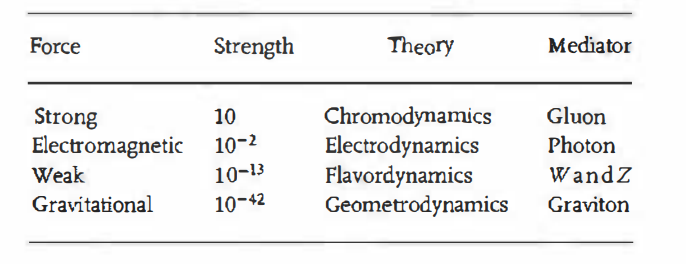
\includegraphics[scale=1]{table1.png}
    \caption{Comparison of the strength magnitude of the four fundamental forces}
    \label{fig:four-forces}
\end{figure}

Each of these forces has a mathematical description for the physical systems of these interactions using the Quantum Field Theory (QFT). The one that describes systems under the electromagnetic force is called Quantum Electrodynamics (QED) this force dictates the electronic structure of atoms being the low energy manifestation of the electromagnetic theory. For the strong force Quantum Chromodynamics (QCD) is the fundamental theory of strong interactions, this force is responsible for maintaining protons and neutrons together in the atomic nucleus. For the weak interactions there is no particular name in the same way as the previous two, this force is carried by all quarks and leptons and is responsible for the $\beta$ Decay of some radioactive isotopes and nuclear processes of the sun. \cite{mppthomson}   


Almost all the physical phenomena can be explained with only the electron, the electron neutrino, the proton and the neutron interacting with the electromagnetic force, the strong force and the weak one. When higher levels of energy are present new particles are observed, all of this is known as the elementary particles which are embodied in the standard model of particle physics that is by far the best theoretical model that describes the interaction of these elementary particles. They are divided into two categories the bosonic sector and the fermionic sector.  \cite{mppthomson}   


\begin{figure}[h]
    \centering
   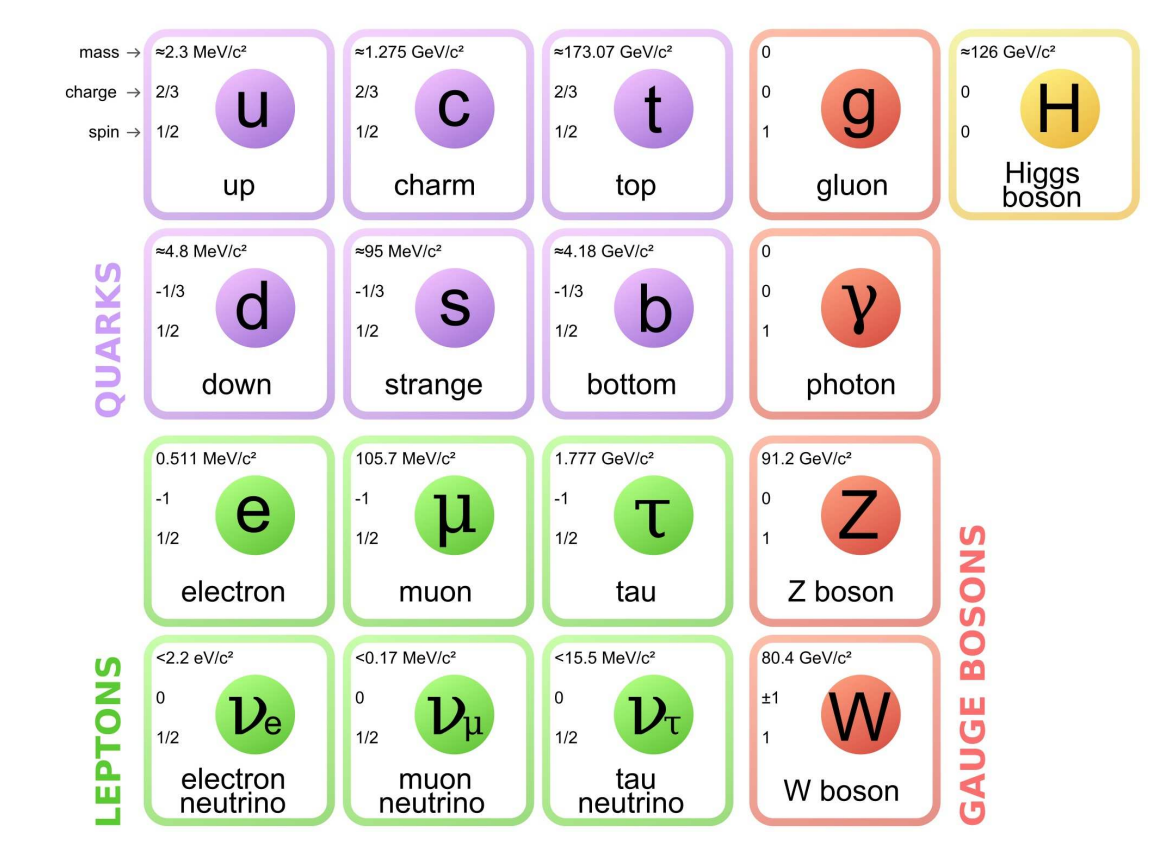
\includegraphics[width=1\textwidth]{sm.png}
    \caption{The standard model of particle physics.\cite{pic2}}
    \label{fig:four-forces}
\end{figure}


The fermionic sector contains particle the particles that make up all known matter in the universe and is divided into the leptons and the quarks, both of these particles are divided into three generations, each generation being heavier than the one before. For the leptons we have the electron and It's neutrino for the first generation, the second generation is the $\mu$ and It's neutrino and the third one is the $\tau$ with It's neutrino. In the case of quarks we have the quark up and the quark down for the first generation, the second generation we have the quark charm and the quark strange and for the third generation we have the quark top and the quark bottom. The bosons are the mediator particles, the photon, the gluon, the bosons W+, W- and the boson Z. There is also de Higgs boson which is the responsible to give mass to the other SM particles  


One of the main sources to obtain elementary particles is particle accelerators, in this you accelerate a particle into high energy and smash them with a target, with the proper  arrangements of magnets you can study the debris from the collision, to produce heavy particles you need higher level of energy to the collision.

\section{Large Hadron Collider}

The Large Hadron Collider (LHC) is the biggest and powerful particle accelerator in the world at this moment. It is a 27 kilometers ring of superconducting magnets, this magnets mantain the particle in orbits meanwhile meanwhile radio frequency cavities increase the particles energies to obtain speeds that are close to the light speed before collisions. These particles are introduced into the accelerator as beams that are traveling in opposing directions in tubes that are kept at ultrahigh vacuum. All of this with the help of a electromagnetic field made by the electromagnets operating in superconduct state at low temperatures thanks to liquid helium this particles are guided across the whole accelerator. \cite{LHC}


\begin{figure}[h]
    \centering
   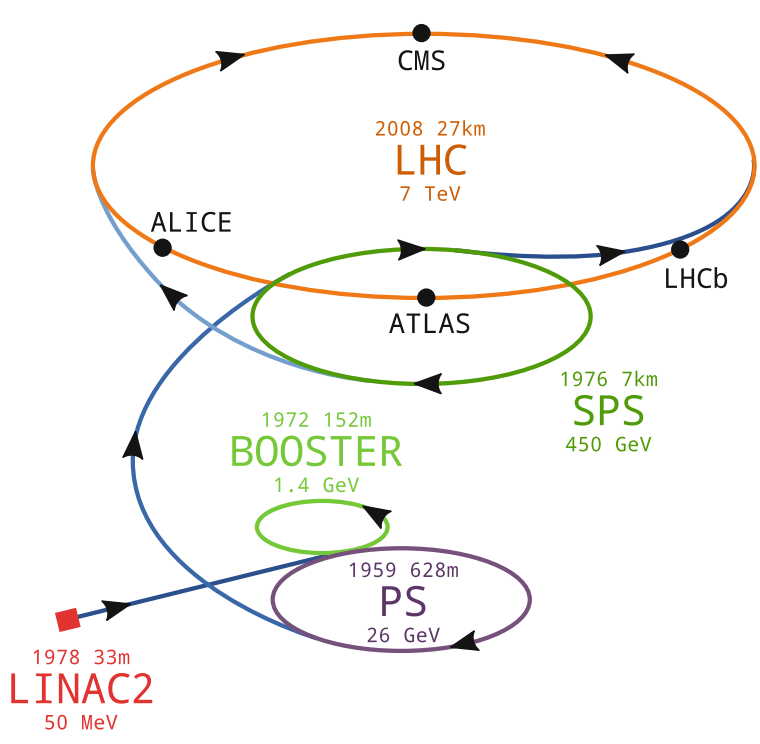
\includegraphics[width=1\textwidth]{LHC.png}
    \caption{The accelerator facility at cern for the LHC. \cite{lhcpic}}
    \label{fig:LHC}
\end{figure}




The LHC is part of an accelerator complex in CERN that is a succession of different machines that increase the energy of the beam of particles before passing into the next one on the sequence the particles at last are introduced on the LHC which is the last element in the sequence. The particles start at the linear accelerator 4 (Linac4) which is the source of the protons beams, hydrogen ions to 160 MeV to enter the Proton Synchroton Booster (PSB), this is were the hydrogen loses Its two electrons leaving only protons and accelerating the beam to 2 GeV  and then are injected into the Proton Synchroton (PS). Here the protons are accelerated up to 26 GeV and then they are sent into the Super Proton Synchroton (SPS) here they are accelerated up to 450 GeV. Finally they're fintroduced into two beams pipes on the LHC, it takes about 4 minutes and 20 seconds to fill the LHC rings reaching energies up to 6.5 TeV. There is a total of four collisions points and this is where the detectors are located Alice, Atlas, CMS and LHCb, in the collision the total energy is of 13.6 TeV. \cite{LHCII}

The LHC has been working since 2009 with the discovery of the Higgs Boson on 2012 and looking for new physics. It has been working on different periods called Runs, Run 1 was on the period of (2009-2013), Run 2 was on (2015-2018). Run 3 is currently on going since 2022. 

\section{Cross Section}

%The performance of a collider is determined by the beam energy and the luminosity, in order to compute the luminosity we need to define the cross section of the accelerator first this is for the calculation of the interest rates, which have to take in consideration the flux which is defined as the number of particles crossing a unit are per unit of time, the cross section is denoted by $\sigma$ and every scattering process has a cross section $\simga_{i}$ but the one that we are interested on is the total cross section which is the sum of all the $\simga_{i}$. 

The performance of a collider is determined by the beam energy and the luminosity. First we are going to define the cross section in a classical way, the cross section area is parameter of interest that measures the size of a target, this cross sectional area is presented to a stream of incoming particles, similar to the case of the scattering in elementary particles, if you fire a electron beam into a proton, the parameters of interest are the size of the proton and the cross sectional area $\sigma$ that presents the incident beam. 

This collision differs to the classic case in some ways, first you could call the proton target soft since It's not a possible collision, instead as the electron becomes closer it gradually deflects due to the electromagnetic interactions. There are two main interactions each that can happen in this case, the first one the elastic scattering, here neither the electron or the proton changes their internal states. The other one the inelastic scattering where the target absorbs energy. In the case of the later the cross section $\sigma_{total}$ would be the sum of all the possible inelastic process $\sigma_{i}$ as shown in equation (1.1). 

\begin{equation}
\sigma_{tot} = \Sigma^{n}_{i=1} \sigma_{i}
\end{equation}

Each of this cross sections depends typically in the velocity of the incident particle, It's expected that the cross section would be proportional to the time that the incident particle spends close to Ithe target which means that $\sigma$ is inversely proportional to the velocity. This behavior is altered close to the region of energy that particles involved to interact forming a short lived semi-state before breaking apart, things like this make the cross section for elementary particles different to the classic one. 

To understand an elastic process lets consider an electron beam which encounters a potential and scatters at the angle $\theta$, this scatter is angle is a function of a impact parameter b the distance by which this particle would have missed the scattering center had it continued on its original trajectory. The form of $\theta(B)$ depends on the potential and the smaller the impact parameter b, larger the deflection. If the particle comes with an impact parameter between b and b + db it will merge in a angle between $\theta$ and $\theta + d\theta$ and even in a more general case if it passes through a infinitesimal area $d\sigma$ it will scatter into a corresponding solid angle $d\Omega$, the larger $d\sigma$ is the larger $d\Sigma$ the proportionality factor between these two is called the differential cross section D this can be illustrated in the next image: 

\begin{figure}[h]
    \centering
   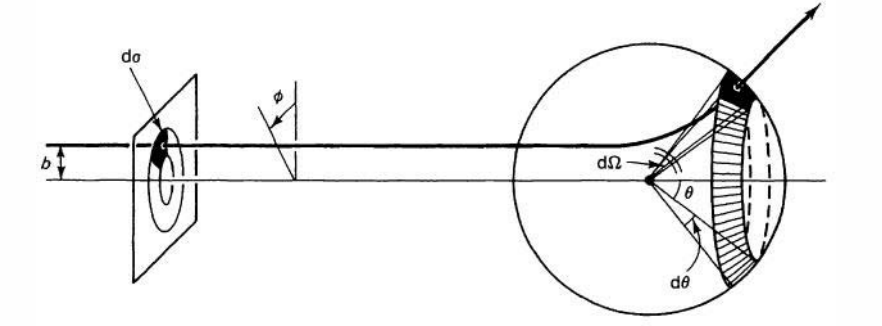
\includegraphics[width=1\textwidth]{cross1.png}
    \caption{Particle scattering}
    \label{fig:cross}
\end{figure}

The relation between $d\sigma$ and $d\Omega$ is:

\begin{equation}
d\sigma = D(\theta)d\Omega
\end{equation}

Supposing a beam of incoming particles with a value F that is associated with the number of particles passing down the line per unit of time and per unit of area $dN = F d\sigma $ is the number of particles per unit time passing trough area $d\sigma$ and hence also the number per unit of time scattered into solid the solid angle $d\Omega$

\begin{equation}
dN = F d\sigma = fD(\theta) d\Omega 
\end{equation}

This is a classical description of scattering and could be seen as the one who controls the number of particles going through the detector also determined the solid angle. 
%The define of cross section can be understand in a situation where a single particle is travelling to a velocity $v _{a}$in a region defined by A, which contains $n_{b}$ particles of a particle type b moving to a velocity $v_{b}$ in the opposite direction of $v_{a}$ if in a time $\delta t$  the particle a cross a region contained a total of $nb(v_{a} + v_{b})A\delta t$ particles of type b, the interaction probability can be obtained from the effective total cross seciotanl area divided by A which can be seen as the probability of that hte incident particles passes through one of the region of area $\sigma$ around each of the $\delta N$ particles then we can talk about the total rate being: 

%\begin{equation}
%rate = flux x number of target particles x cross section
%\end{equation}

%And we can define the cross section as follow:

%\begin{equation}
%\sigma = \frac{number of interaction per unit of time per target particle}{incident flux}
%\end{equation}

\section{Luminosity}

The performance of a collider is determined by the beam energy and the luminosity, the luminosity is a key parameter in particle colliders is a quantity that measures the ability of a particle accelerator to produce a required number of interactions\cite{Lum} 

\begin{equation}
R = L \cdot \sigma_{p} 
\end{equation}

In which R is the number of colision events per second or rate, the $\sigma_{p}$ is the cross section which in the quantum case is a probability of interaction which can be obtained from the standar model of particle physics and L the instantanious luminosity. The unity of L is  $cm^{-2} s^{-1}$ a higher luminosity means greater probability that the particles will collide and produce the desired interactions, luminosity can be increased then in two ways, packing more particles into the beams or focusing this beams more.  

To compute the luminosity there is a few things that need to be taken in consideration. First the density distribution of each beam in the transverse and longitudinal plane, with the two beams moving towards each other, the position and the time as the cross each other also need to be considered and calling the distance to the collision point $s_{0}$. The figure (1.5) shows two beams colliding which depends on a variety of factors:


\begin{figure}[h]
    \centering
    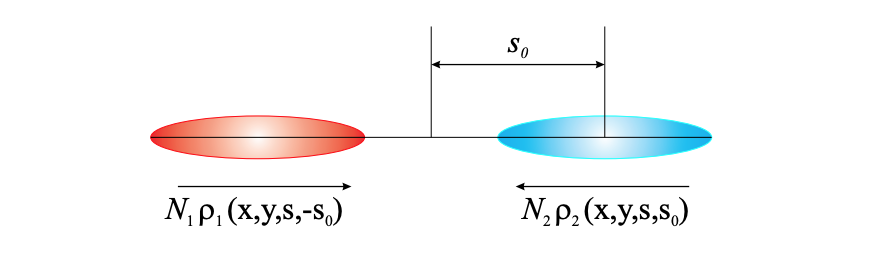
\includegraphics[width=1\textwidth]{lumi.png}
    \caption{Two beams colliding}
    \label{fig:beamslumi}
\end{figure}


Following this we can write the integral for luminosity, in principle each of the distributions is different and we can write the overlap integral as follow:
%$K = sqrt{(v_{1} - x_{2})^{2} - \frac{(v_{1} x v_{2})^{2}}{c^{2}} }

\begin{equation}
 L = 2N_{1}N_{2}fN_{b} \int \int \int \int^{\infty}_{-\infty}  \rho_{1x} (x) \rho_{1y}(y) \rho_{1s} (s-s_{0}) \rho_{2x}(x) \rho_{2y}(y) \rho_{2s} (s+s_{0}) dxdydsds_{0}  
\end{equation}

With N1 and N2 being the bunch intensity, f the revolution frequency, $N_{b}$ the number of colliding bunches, $\rho_{1}$ and $\rho_{2}$ time dependent beam density distribution functions and assuming the densities are uncorrelated in all planes.  \cite{Lumvdm}

For solving this integral one should known all distributions and an analytical solutions might not be possible and numerical numerical integration might be required.


The instantaneous luminosity is important  but the final important number is called integrated luminosity. The integrated luminosity considers the total number of events during a data period is defined as: 

\begin{equation}
 L_{int} = \int L (t') dt' 
\end{equation}

This is related directly to the number of observed events $L_{int} \cdot \sigma_{p}$.


In the LHC there are various ways to measure the luminosity, in the CMS there are various of them, the Pixel Luminosity Telescope, the BCM1F, the radiation monitoring system for environment & safety, the muon drift tubes, the forward hadron calorimeter and the Pixel Cluster Counting (PCC). 

The PCC luminometer method consist in counting the average number of pixel clusters on the detector to measure luminosity. This occurs during a zero bias event, an event that is triggered by requiring only that two proton bunches cross at the CMS interaction point. Giving that the number of pixels is really big the probability that a pixel is being hit by two different tracks by the same bunch crossing is really small. The mean number of pixel clusters in a simulated zero bias event is in the order of 100 per pp collision. The number of pixel clusters per bunch crossing is linearly dependent on pileup and therefore an accurate measure of the instantaneous luminosity.\cite{PCC1} The mean number of pixel cluster per trigger is 


\begin{equation}
<N_{cluster}> = <N_{Cluster/Interaction}> <N_{interaction}> = <N_{Cluster/interaction}> \mu 
\end{equation}

here the $\mu$ is the number of interactions, now we define the collision rate in the equation (1.8):

\begin{equation}
R = \mu * f_{LHC} = L * \sigma_{p}
\end{equation}

Solving for $\mu$ we got:

\begin{equation}
\mu = \frac{L * \sigma_{p}}{f_{LHC}} 
\end{equation}

And combining equation (1.7) and (1.9) we obtain:

\begin{equation}
<N_{cluster}> = \frac{\sigma_{p}* L}{f_{LHC}}  <N_{Cluster/Interaction}>
\end{equation}

Here, the value of $N_{cluster}$ is the mean number of pixel clusters on the pixel detector during a zero bias trigger at a head on period, the value of $\sigma_{cluster}$ can be obtained using the Van Der Meer scan and from the equation (2.3) we can obtain the luminosity from \cite{PCC2}


There have been different luminosities reached on the LHC for the Run 1 a luminosity of $0.77 x 10^{34} cm^{-2} s^{-1}$ was reached and a integrated luminosity of 25 $fb^{-1}$  with a precision of 2.0\% for the first part and second part of the Run 2 the luminosity measured was of 38.4 $fb^{-1}$ with a precision of 1.3\% and 78$fb^{-1}$ respectively\cite{LHClum}.  The figure (1.6) show shows the integrated luminosity for the CMS experiment on different years.  

\begin{figure}[h]
    \centering
     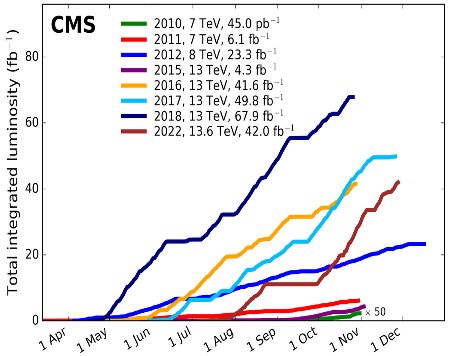
\includegraphics[scale=1.25]{integratedlum.png}
     \caption{Integrated luminosity at CMS.}
    \label{fig:CMS-Luminosity}
\end{figure}

